\documentclass[9pt,twocolumn,twoside]{gsajnl_modified}
% Use the documentclass option 'lineno' to view line numbers

\usepackage[htt]{hyphenat}  % https://tex.stackexchange.com/a/543
\usepackage[export]{adjustbox}
\usepackage{xurl}
\usepackage{stfloats}
\usepackage[leftcaption]{sidecap}
\sidecaptionvpos{figure}{t}

\renewcommand{\topfraction}{0.9}	% max fraction of floats at top
    \renewcommand{\bottomfraction}{0.8}	% max fraction of floats at bottom
    %   Parameters for TEXT pages (not float pages):
    \setcounter{topnumber}{2}
    \setcounter{bottomnumber}{2}
    \setcounter{totalnumber}{4}     % 2 may work better
    \setcounter{dbltopnumber}{2}    % for 2-column pages
    \renewcommand{\dbltopfraction}{0.9}	% fit big float above 2-col. text
    \renewcommand{\textfraction}{0.07}	% allow minimal text w. figs
    %   Parameters for FLOAT pages (not text pages):
    \renewcommand{\floatpagefraction}{0.7}	% require fuller float pages
	% N.B.: floatpagefraction MUST be less than topfraction !!
    \renewcommand{\dblfloatpagefraction}{0.7}	% require fuller float pages

\newcommand\jdbcomment[1]{\textcolor{red}{[#1]}}
\newcommand\rancomment[1]{\textcolor{blue}{[#1]}}

\title{Fitness effects of mutations to SARS-CoV-2 proteins}

\author[*]{\Large Jesse D. Bloom$^{1,2,3^*}$ and Richard A. Neher$^{4,5}$}

\affil[1]{Basic Sciences and Computational Biology, Fred Hutchinson Cancer Center

}
\affil[2]{Department of Genome Sciences, University of Washington

}
\affil[3]{Howard Hughes Medical Institute

}
\affil[4]{Biozentrum, University of Basel

}
\affil[5]{Swiss Institute of Bioinformatics

}

\keywords{}

\runningtitle{} % For use in the footer
\runningauthor{}

\begin{abstract}
Knowledge of the fitness effects of mutations to SARS-CoV-2 can inform assessment of new variants, design of therapeutics resistant to escape, and basic understanding of the function of viral proteins.
However, experimentally determining the effects of mutations is challenging: we lack tractable lab assays for many SARS-CoV-2 proteins, and comprehensive deep mutational scanning has been applied to only two of the virus's proteins.
Here we develop an approach that leverages millions of publicly available SARS-CoV-2 sequences to estimate the effects of mutations.
We first calculate how many times each mutation is expected to occur along the SARS-CoV-2 phylogeny in the absence of selection. 
We then compare these expected counts to the actual counts to estimate the effect of each mutation.
These estimates correlate well with deep mutational scanning measurements.
For most genes, synonymous mutations are nearly neutral, stop-codon mutations are deleterious, and amino-acid mutations have a range of effects.
However, some viral accessory proteins are under little to no selection.
To enable our estimates to be easily used, we provide interactive visualizations (\url{https://jbloomlab.github.io/SARS2-mut-fitness/}).
The framework we describe is applicable to any virus for which the number of available sequences is sufficiently large that each neutral mutation independently occurs many times.
\end{abstract}

\begin{document}

\maketitle
\thispagestyle{firststyle}
%\marginmark
\firstpagefootnote

\correspondingauthoraffiliation{}{*\href{mailto:jbloom@fredhutch.org}{jbloom@fredhutch.org} or \href{mailto:richard.neher@unibas.ch}{richard.neher@unibas.ch}}
\vspace{-33pt}% Only used for adjusting extra space in the left column of the first page

\lettrine[lines=2]{\color{color2}T}{}he rapid evolution of SARS-CoV-2 has led to the repeated emergence of viral variants with enhanced transmissibility, escape from anti-viral therapeutics, or reduced recognition by immunity~\citep{harvey2021sars,abdool2021new}.
To anticipate and mitigate this evolution, the scientific community has launched major efforts to assess the risk of new viral variants~\citep{degrace2022defining} and create therapeutics that target constrained regions of the virus where resistance is less likely to evolve~\citep{moghadasi2022,iketani2022multiple,hiscox2021shutting}.
Both efforts require determining how specific mutations affect the fitness of the virus.

Unfortunately, experimentally determining the effects of mutations remains challenging for most SARS-CoV-2 proteins.
For spike, tractable laboratory assays have identified key functional and antigenic mutations~\citep{weisblum2020escape,harvey2021sars}, and enabled deep mutational scanning measurements of how most mutations affect receptor binding, cellular infection, and antibody recognition~\citep{starr2020deep,dadonaite2022pseudovirus,greaney2021complete,cao2022imprinted}.
These experimental data are valuable for assessing new spike variants~\citep{degrace2022defining,greaney2022antibody,tzou2022coronavirus} and informing development of antibody therapeutics with greater resistance to escape~\citep{starr2021sars,rappazzo2021broad,cao2022rational}.
But most other SARS-CoV-2 proteins lack comparably tractable laboratory assays, despite clearly contributing to viral fitness~\citep{thorne2022evolution,syed2021rapid,mcgrath2022sars} and being the targets of efforts to develop anti-viral drugs~\citep{tao2021sars}.
The only non-spike SARS-CoV-2 protein with large-scale deep mutational scanning data is Mpro~\citep{flynn2022,iketani2022functional}.

An alternative to experiments is to estimate the effects of mutations by analyzing natural viral sequences.
The amount of data available for such analyses has increased dramatically over the last few years with the full-genome sequencing of SARS-CoV-2 from millions of human infections.
So far analyses of these sequences have focused on analyzing expanding viral clades to identify mutations that mediate immune escape or increase transmissibility~\citep{obermeyer2022analysis,lee2022inferring,maher2022predicting}.
The basic idea is that mutations that repeatedly appear near the base of clades that increase in relative frequency are likely beneficial to the virus.
However, only a small minority of all possible mutations are beneficial, with most being nearly neutral or deleterious.
For purposes such as identifying functionally constrained drug targets or understanding the function of viral proteins, it is important to accurately estimate the effects of neutral or deleterious mutations as well as beneficial ones.
% \jdbcomment{Richard, I could not quite figure out how to fit in \citep{strelkowa2021clonal}, let me know if you have ideas.}

Here we develop a new approach that uses natural sequences to estimate the effects of mutations.
Our basic insight is that there are now so many SARS-CoV-2 sequences that all non-deleterious single-nucleotide mutations are expected to independently occur many times along the observed phylogenetic tree.
We therefore first calculate the number of expected occurrences of each mutation based on the neutral mutation spectrum of SARS-CoV-2 estimated from four-fold degenerate synonymous sites~\citep{bloom2022evolution}.
We then compare these expected occurrences to the actual occurrences in the SARS-CoV-2 tree to estimate the effect of each mutation.
The resulting estimates correlate well with existing deep mutational scanning data.
Most viral proteins have regions that are under strong selective constraints.
However the accessory proteins mostly show only weak selection against amino-acid and even stop-codon mutations.
Overall, our work demonstrates a new approach to determine the effects of mutations, and provides detailed maps of functional constraint across the SARS-CoV-2 proteome.

\section{Results}

\subsection{Estimating fitness from actual versus expected mutation counts}

\begin{figure*}
{\bf \Large A \hspace{0.47\linewidth} B}

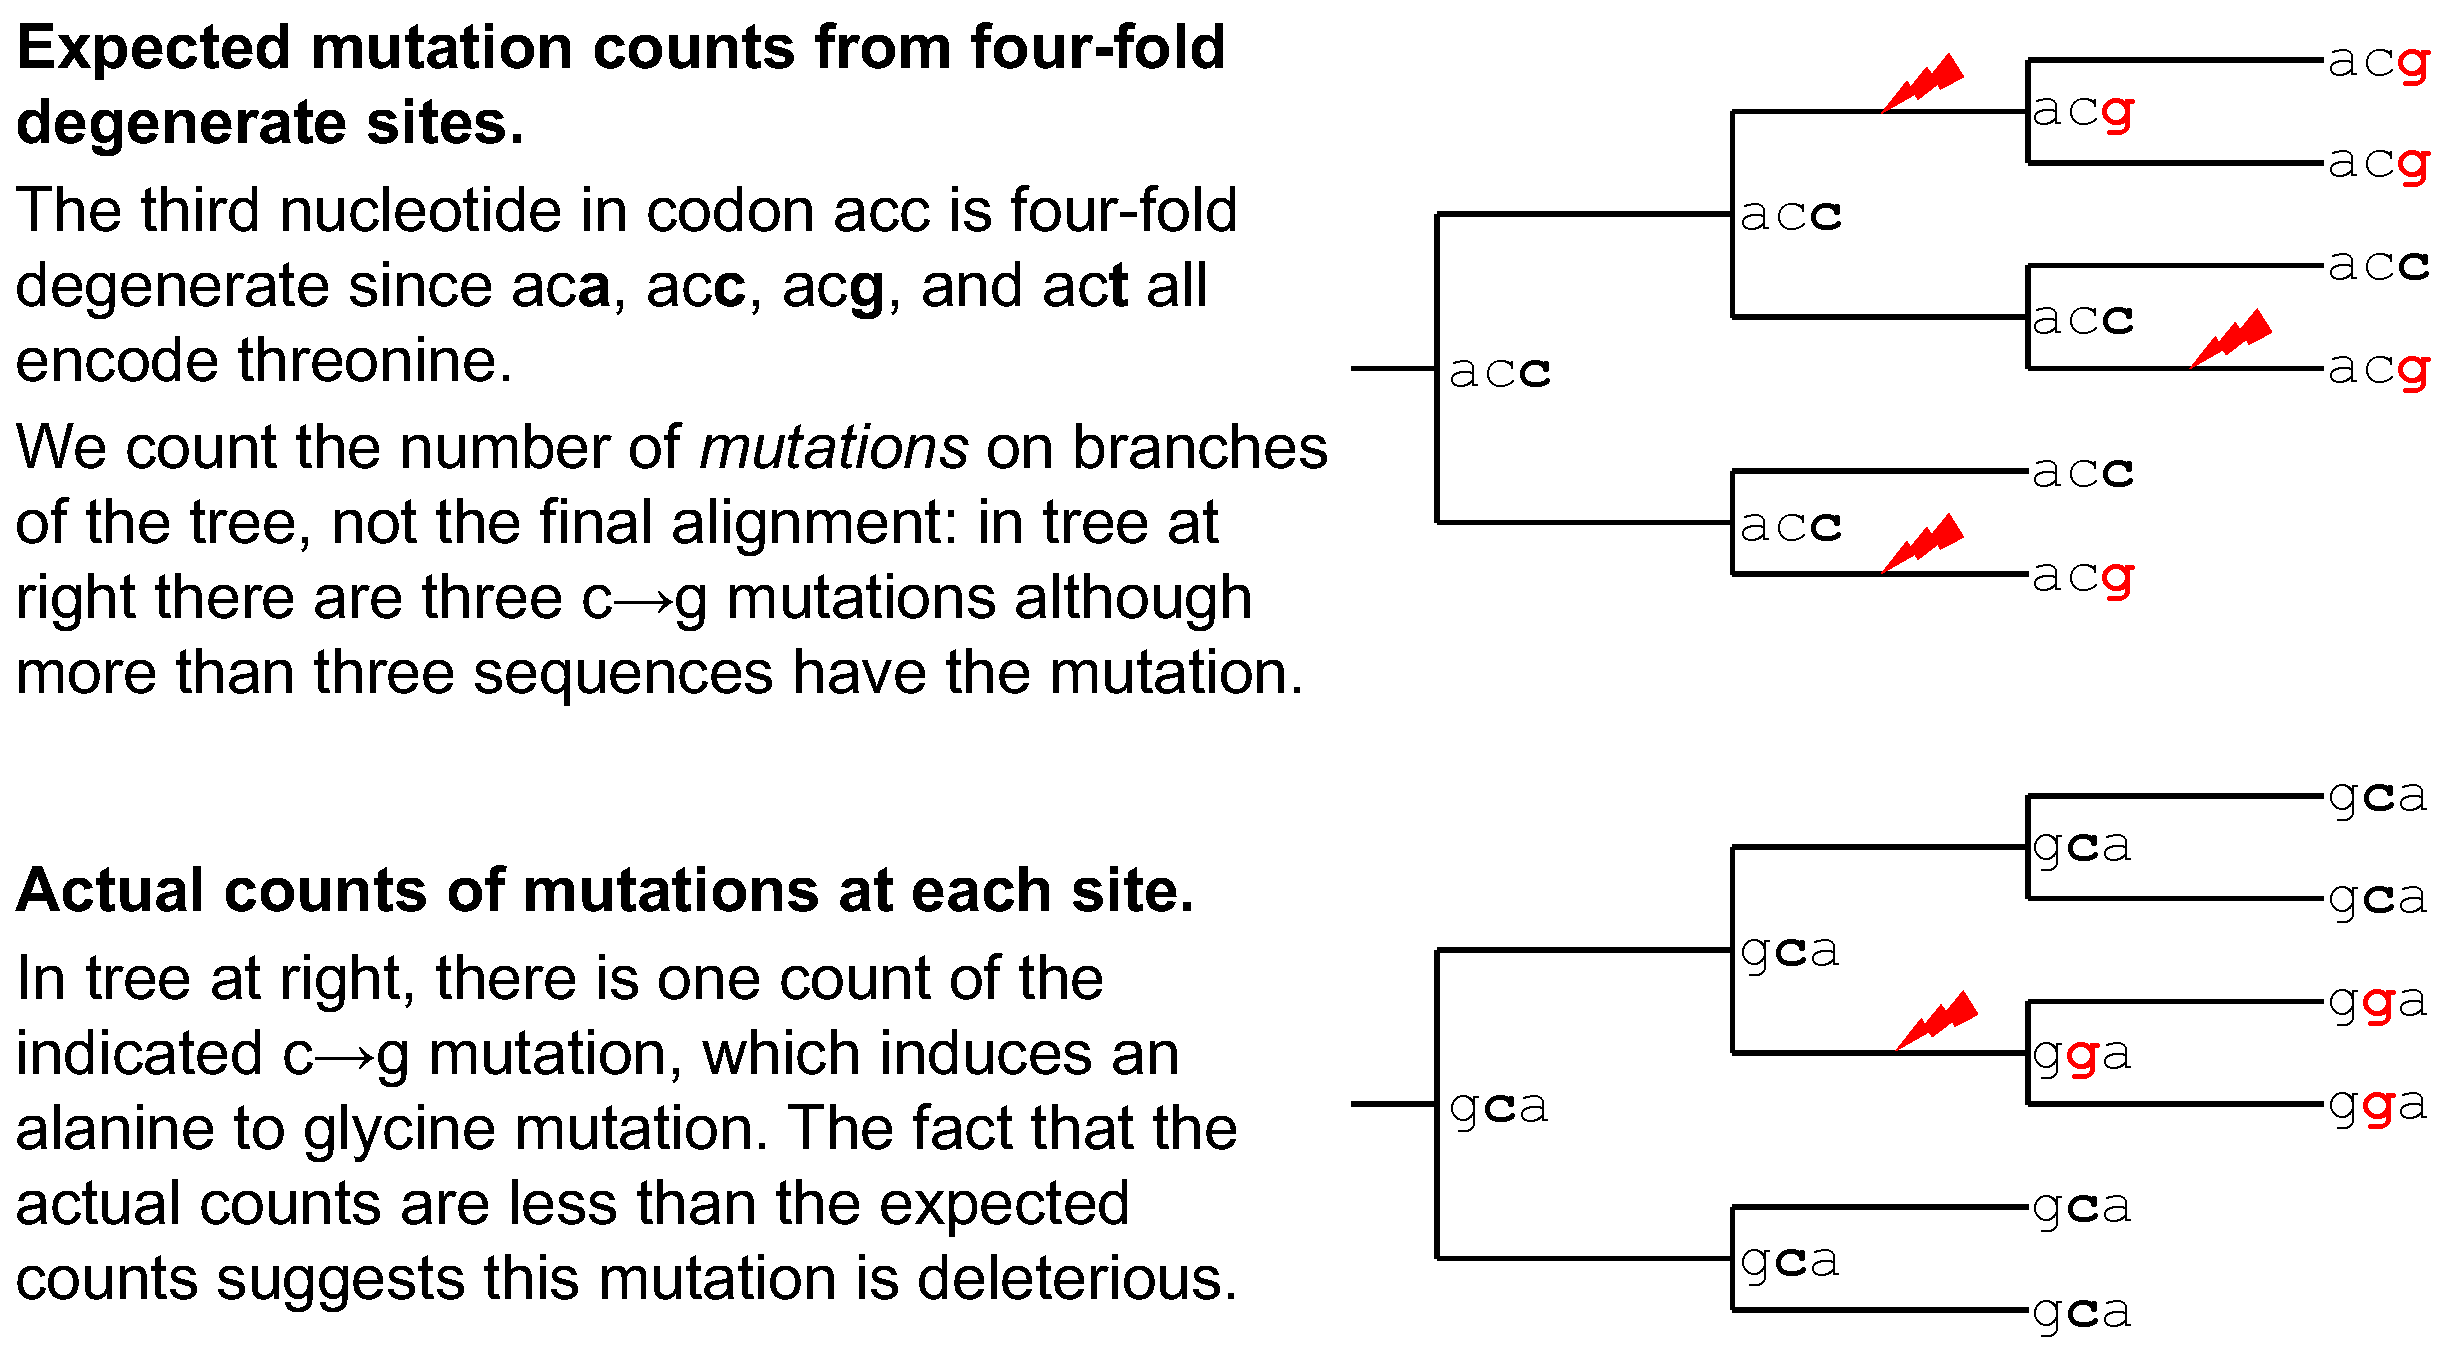
\includegraphics[width=0.48\linewidth,valign=t]{figs/schematic/schematic.pdf}
\hspace{0.02\linewidth}
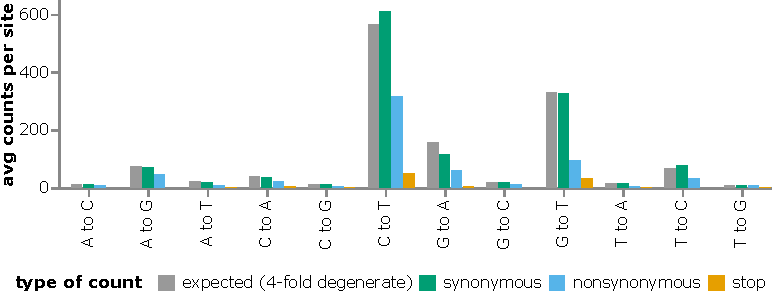
\includegraphics[width=0.5\linewidth,valign=t]{figs/avg_counts.pdf}
\caption{
Expected versus actual counts of mutations.
{\bf (A)}
The number of expected counts of each type of nucleotide mutation is computed from four-fold degenerate sites, and then compared the actual counts of each mutation.
{\bf (B)}
Expected versus actual counts for each nucleotide mutation type aggregated across all viral clades and averaged across all sites where the mutation is four-fold degenerate, synonymous (including four-fold degenerate), nonsynonymous, or introduces a stop codon.
See \url{https://jbloomlab.github.io/SARS2-mut-fitness/avg_counts.html} for an interactive version of panel B that enables mouseovers to read off specific values.
\label{fig:expected_vs_actual}
}
\end{figure*}

To determine how many times each mutation is expected to be observed, we used the pre-built UShER tree~\citep{mcbroome2021daily,turakhia2021ultrafast,lanfear2020} of $\sim$6.5-million public SARS-CoV-2 sequences to count nucleotide mutations at four-fold degenerate sites~\citep[Figure~\ref{fig:expected_vs_actual}A;][]{bloom2022evolution}.
Because mutations at such sites never alter the amino-acid sequence, these counts reflect the mutation process in the absence of protein-level selection (see Discussion for caveats about nucleotide-level selection).
The expected counts of a mutation from nucleotide $x$ to $y$ is simply the average count of this type of mutation across all four-fold degenerate sites with parental identity $x$.
Importantly, we count independent \emph{occurrences} of each mutation along the branches of the tree, not the sequences with the mutation in the final alignment (Figure~\ref{fig:expected_vs_actual}A.
We also compute expected counts separately for each SARS-CoV-2 clade to account for shifts in mutation spectrum~\citep{bloom2022evolution,ruis2022mutational}, and apply quality-control steps to remove spurious mutations (see Methods).

The expected counts per mutation (summed across all viral clades) vary with mutation type, ranging from $\sim$500 for \texttt{C$\rightarrow$T} to only $\sim$8 for \texttt{T$\rightarrow$G} mutations (Figure~\ref{fig:expected_vs_actual}B).
This variation is because the SARS-CoV-2 mutation spectrum is highly biased towards specific mutation types~\citep{bloom2022evolution,ruis2022mutational,de2021mutation,neher2022contributions}.

We compared the expected counts to the actual observed counts of mutations averaged across sites (Figure~\ref{fig:expected_vs_actual}).
For synonymous mutations, the expected and actual counts are similar.
But for nonsynonymous and especially stop-codon mutations, the actual counts are substantially lower than the expected counts, reflecting purifying selection for protein function.

The ratio of actual to expected counts for each mutation is related to its effect on viral fitness.
The intuition is straightforward: mutations arise at all sites during viral replication, but viruses with deleterious mutations are less likely to transmit and be observed in sequencing of human SARS-CoV-2.
Therefore, the ratio of actual to expected counts will be one for neutral mutations, and less than one for deleterious mutations.
In the Methods and Appendix, we show that under plausible assumptions about SARS-CoV-2 evolution and sampling intensity (fraction of viruses sequenced), the fitness cost of a deleterious mutation scales roughly inversely with the ratio of actual to expected counts for mutations with costs greater than a few percent.
A key result from this derivation is the dependence on sampling intensity: if all human SARS-CoV-2 were sequenced then our approach would only be sensitive to highly deleterious mutations, but since the actual sampling intensity is $\sim$0.1--1\% the approach can detect mutations with more subtle effects that transmit with reduced efficiency.
We quantify the effect of each mutation as the logarithm of the ratio of actual to expected counts after summing counts for all nucleotides that encode the relevant amino-acid.
The statistical noise is greater for mutations with fewer expected counts: the figures in this paper show mutations with $\ge10$ expected counts unless otherwise noted, with legends linking to interactive plots that enable adjustment of this threshold.

\subsection*{Mutation-effect estimates are robust to subsampling natural sequences, with some evidence of epistasis in spike}

\begin{figure*}
\centering
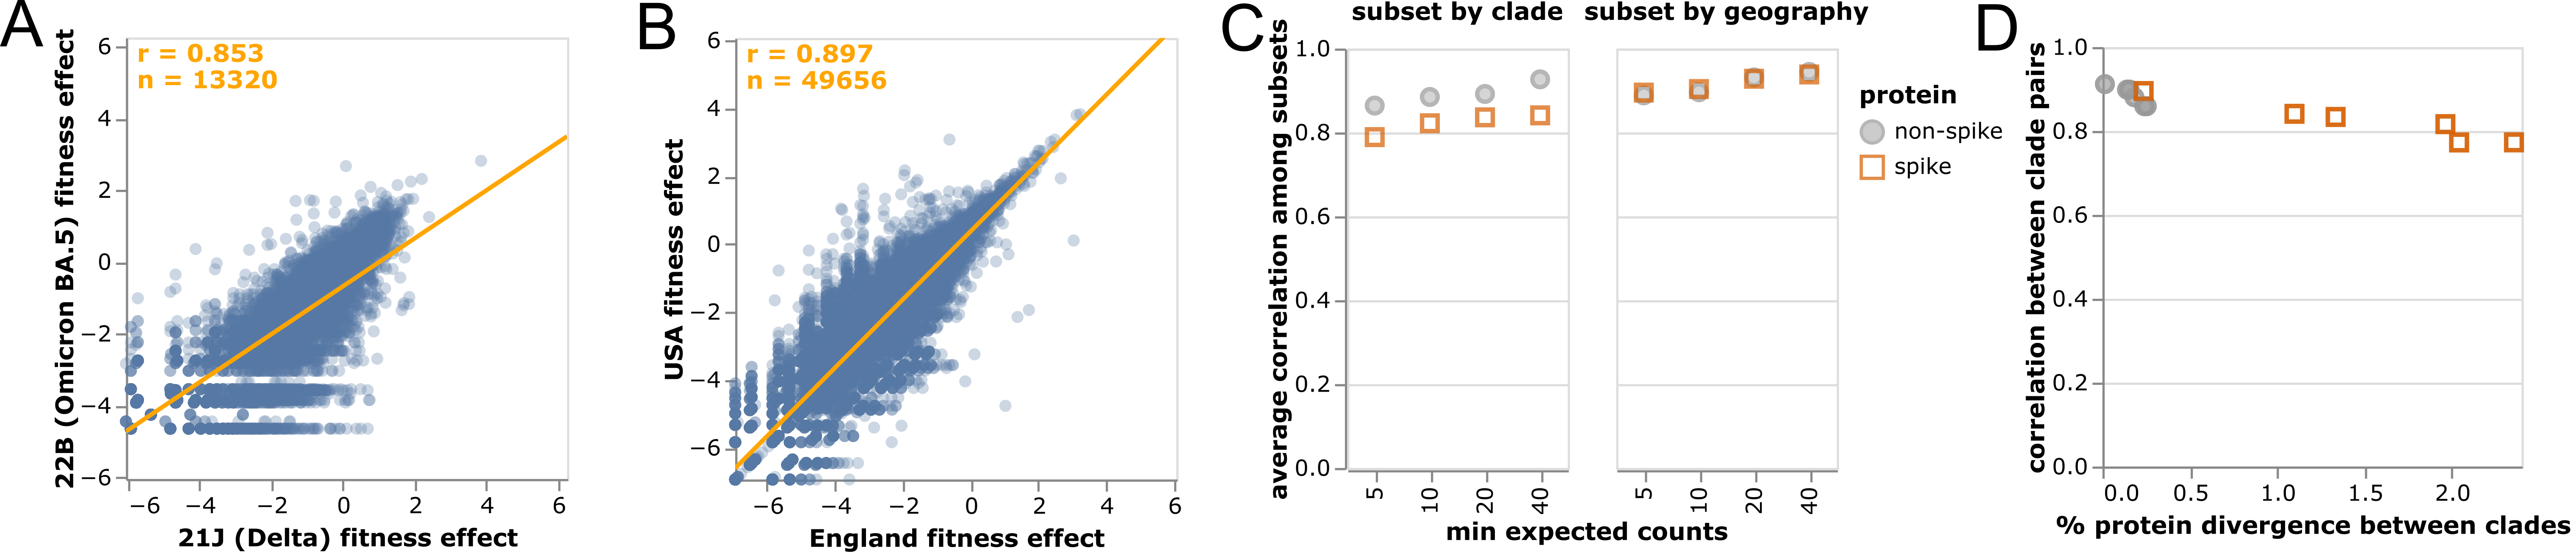
\includegraphics[width=\linewidth]{figs/corr.png}
\caption{
Correlations of mutation fitness effect estimates made using subsets of natural sequences.
Correlations between estimates made {\bf (A)} just using sequences from the Delta or Omicron BA.5 clades or {\bf (B)} just from the USA or England.
Each point is an amino-acid mutation, and orange text at upper left shows the number of mutations and Pearson correlation coefficient.
Only mutations with at least 10 expected counts are shown, which is why panels have different numbers of mutations shown (sequence subsets vary in size).
{\bf (C)} Correlations between clade or geography subsets become higher with an increasingly large threshold for minimum expected counts.
Spike mutations have a worse correlation when subsetting by viral clade (plot shows average correlation over all pairwise combinations of Delta, BA.1, BA.2, and BA.5), but not when subsetting by geography (USA or England).
{\bf (D)} Correlations in estimated mutation effects decline for clades with higher protein divergence, with the effect most noticeable for spike since spike is more diverged among SARS-CoV-2 clades than other viral proteins.
See \url{https://jbloomlab.github.io/SARS2-mut-fitness/clade_corr_chart.html} and \url{https://jbloomlab.github.io/SARS2-mut-fitness/subset_corr_chart.html} for versions of A and B that include all viral clades with at least 500,000 total expected counts (summed across all mutations) and have other interactive options.
\label{fig:corr}
}
\end{figure*}

We computed the correlations among mutation-effect estimates made using subsets of SARS-CoV-2 sequences from different viral clades or geographic locations.
These estimates were well correlated, with some modest variation in estimates across sequence subsets (Figure~\ref{fig:corr}A,B).

The modest variation in estimates from different sequence subsets could have two causes: statistical noise due to finite mutation counts, or real shifts in mutation effects during SARS-CoV-2 evolution~\citep{starr2022shifting,moulana2022compensatory}.
To test for statistical noise, we computed correlations with different thresholds for how many expected counts are required before making an estimate for a mutation (Figure~\ref{fig:corr}C).
Correlations increased with this count threshold, consistent with reduced statistical noise for larger mutation counts.
But the correlation for spike mutations was consistently lower for cross-clade but not cross-geography comparisons (Figure~\ref{fig:corr}C).
The lower cross-clade correlation for spike appears due to epistatic shifts in mutation effects~\citep{starr2022shifting, moulana2022compensatory, pollock2012amino, shah2015contingency} or changes in the selective landscape~\citep{sun2023rapidly} between SARS-CoV-2 clades, since the correlation is lower between clades with higher spike divergence (Figure~\ref{fig:corr}D).

Despite evidence for some shifts in mutation effects in spike, for the rest of this paper we aggregate counts across viral clades to make a single estimate for each amino-acid mutation.
The reason is that the accuracy of the estimates increases with the number of counts for each mutation (Figure~\ref{fig:corr}C), and several mutation types only have enough counts for reasonable estimates when aggregating across viral clades (Figure~\ref{fig:expected_vs_actual}B).
For the purposes of this paper, we deemed it preferable to have more accurate and comprehensive pan-SARS-CoV-2 mutation effect estimates than noisier clade-specific estimates for fewer mutations.
However, the interactive version of Figure~\ref{fig:corr}A linked in the legend enables exploration of mutations with disparate estimates among clades.

\subsection*{Structural and non-structural proteins are under strong purifying selection, but most accessory proteins are not}

\begin{figure*}
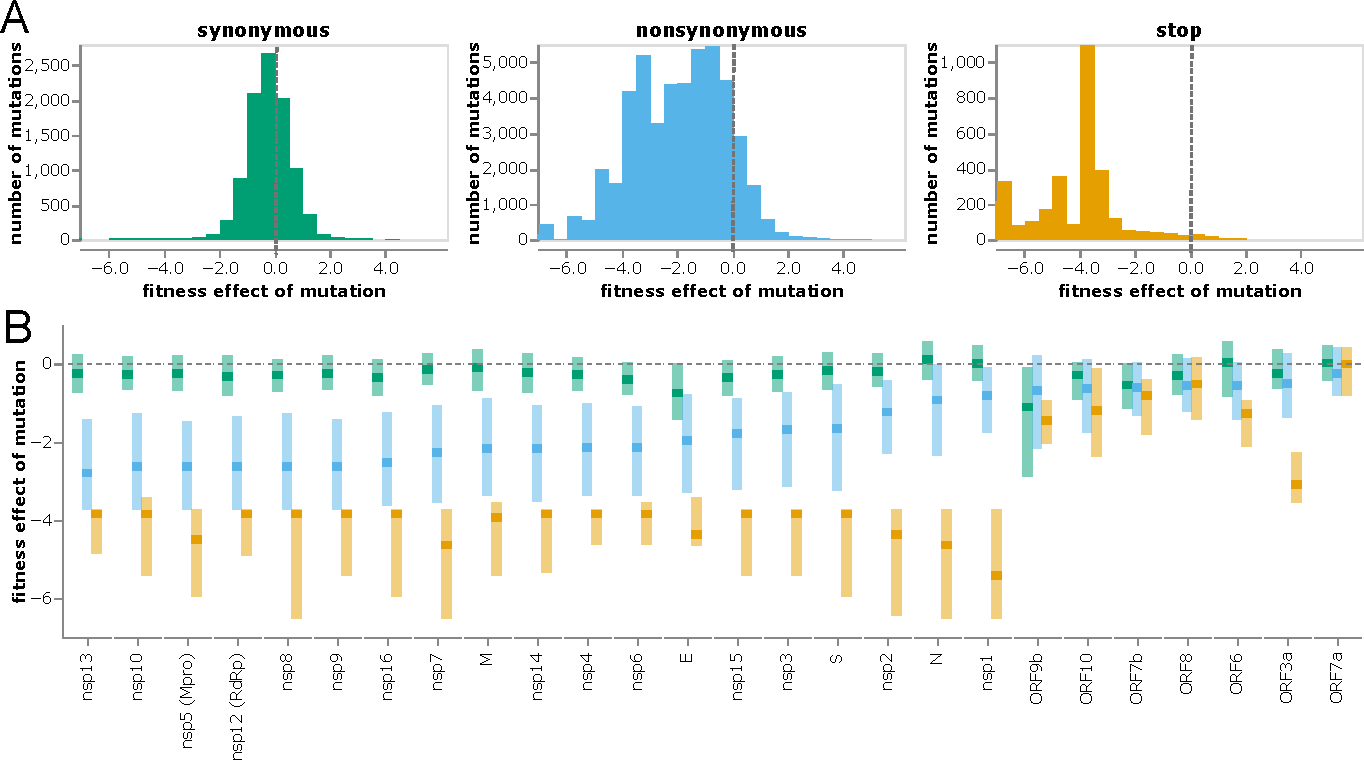
\includegraphics[width=\linewidth]{figs/dist.pdf}
\caption{
Distribution of effects of different classes of mutations.
{\bf (A)}
Histograms of effects of synonymous, nonsynonymous, and stop-codon mutations across all viral genes.
Neutral mutations have effects of zero (dashed gray vertical lines), and deleterious mutations have negative effects.
{\bf (B)}
Effects of each class of mutation for each viral gene.
Dark squares indicate the median effect, and the lighter rectangles span the interquartile range.
Mutation types are color-coded as in panel A.
See \url{https://jbloomlab.github.io/SARS2-mut-fitness/effects_histogram.html} and \url{https://jbloomlab.github.io/SARS2-mut-fitness/effects_dist.html} for plots that allow adjustment of the expected-count cutoff and other interactive options (such as separate histograms for each gene).
\label{fig:dist}
}
\end{figure*}

The distributions of mutation effects concur with biological intuition about how different classes of mutations impact protein function.
Most synonymous mutations are nearly neutral, most stop codons are highly deleterious, and amino-acid mutations range from slightly beneficial to highly deleterious (Figure~\ref{fig:dist}A).

To investigate differences among viral proteins, we computed the distributions of effects separately for each gene (Figure~\ref{fig:dist}B).
SARS-CoV-2 proteins are grouped into three categories: nonstructural (or nsp) proteins, structural proteins (spike, M, N, and E), and accessory proteins (names prefixed with ``ORF'')~\citep{v2021coronavirus}.
The nonstructural and structural proteins are essential, and these proteins show strong selection against stop codons and clear although variable purifying selection against amino-acid mutations (Figure~\ref{fig:dist}B; e.g., nsp13 is under stronger protein-level constraint than nsp1).

However, most accessory proteins are under little constraint (Figure~\ref{fig:dist}B).
Stop-codon and amino-acid mutations to ORF7a and ORF8 are not more deleterious than synonymous mutations.
The lack of deleterious mutations to ORF8 is consistent with the fact that viruses with deletions in this gene have spread in humans~\citep{su2020discovery}.
The only accessory protein under strong purifying selection against stop codons is ORF3a (Figure~\ref{fig:dist}B), for which stop codons in the first ~240 residues are clearly deleterious (Figure~\ref{fig:ORF3a}).
These observations concur with experiments showing SARS-CoV-2 is attenuated by deletion of ORF3a but there is little effect of deleting ORF6, ORF7a, or ORF8~\citep{mcgrath2022sars,silvas2021contribution,liu2022live}.
However, ORF3a's function must be relatively insensitive to its protein sequence, since other than selection against stop codons there is only amino-acid level constraint at a few sites like 135 and 138 (Figure~\ref{fig:ORF3a}).
Observations such as these could help guide experimental studies to better understand protein function.

\subsection*{Mutation-effect estimates correlate with experiments}

\begin{figure*}
\centering
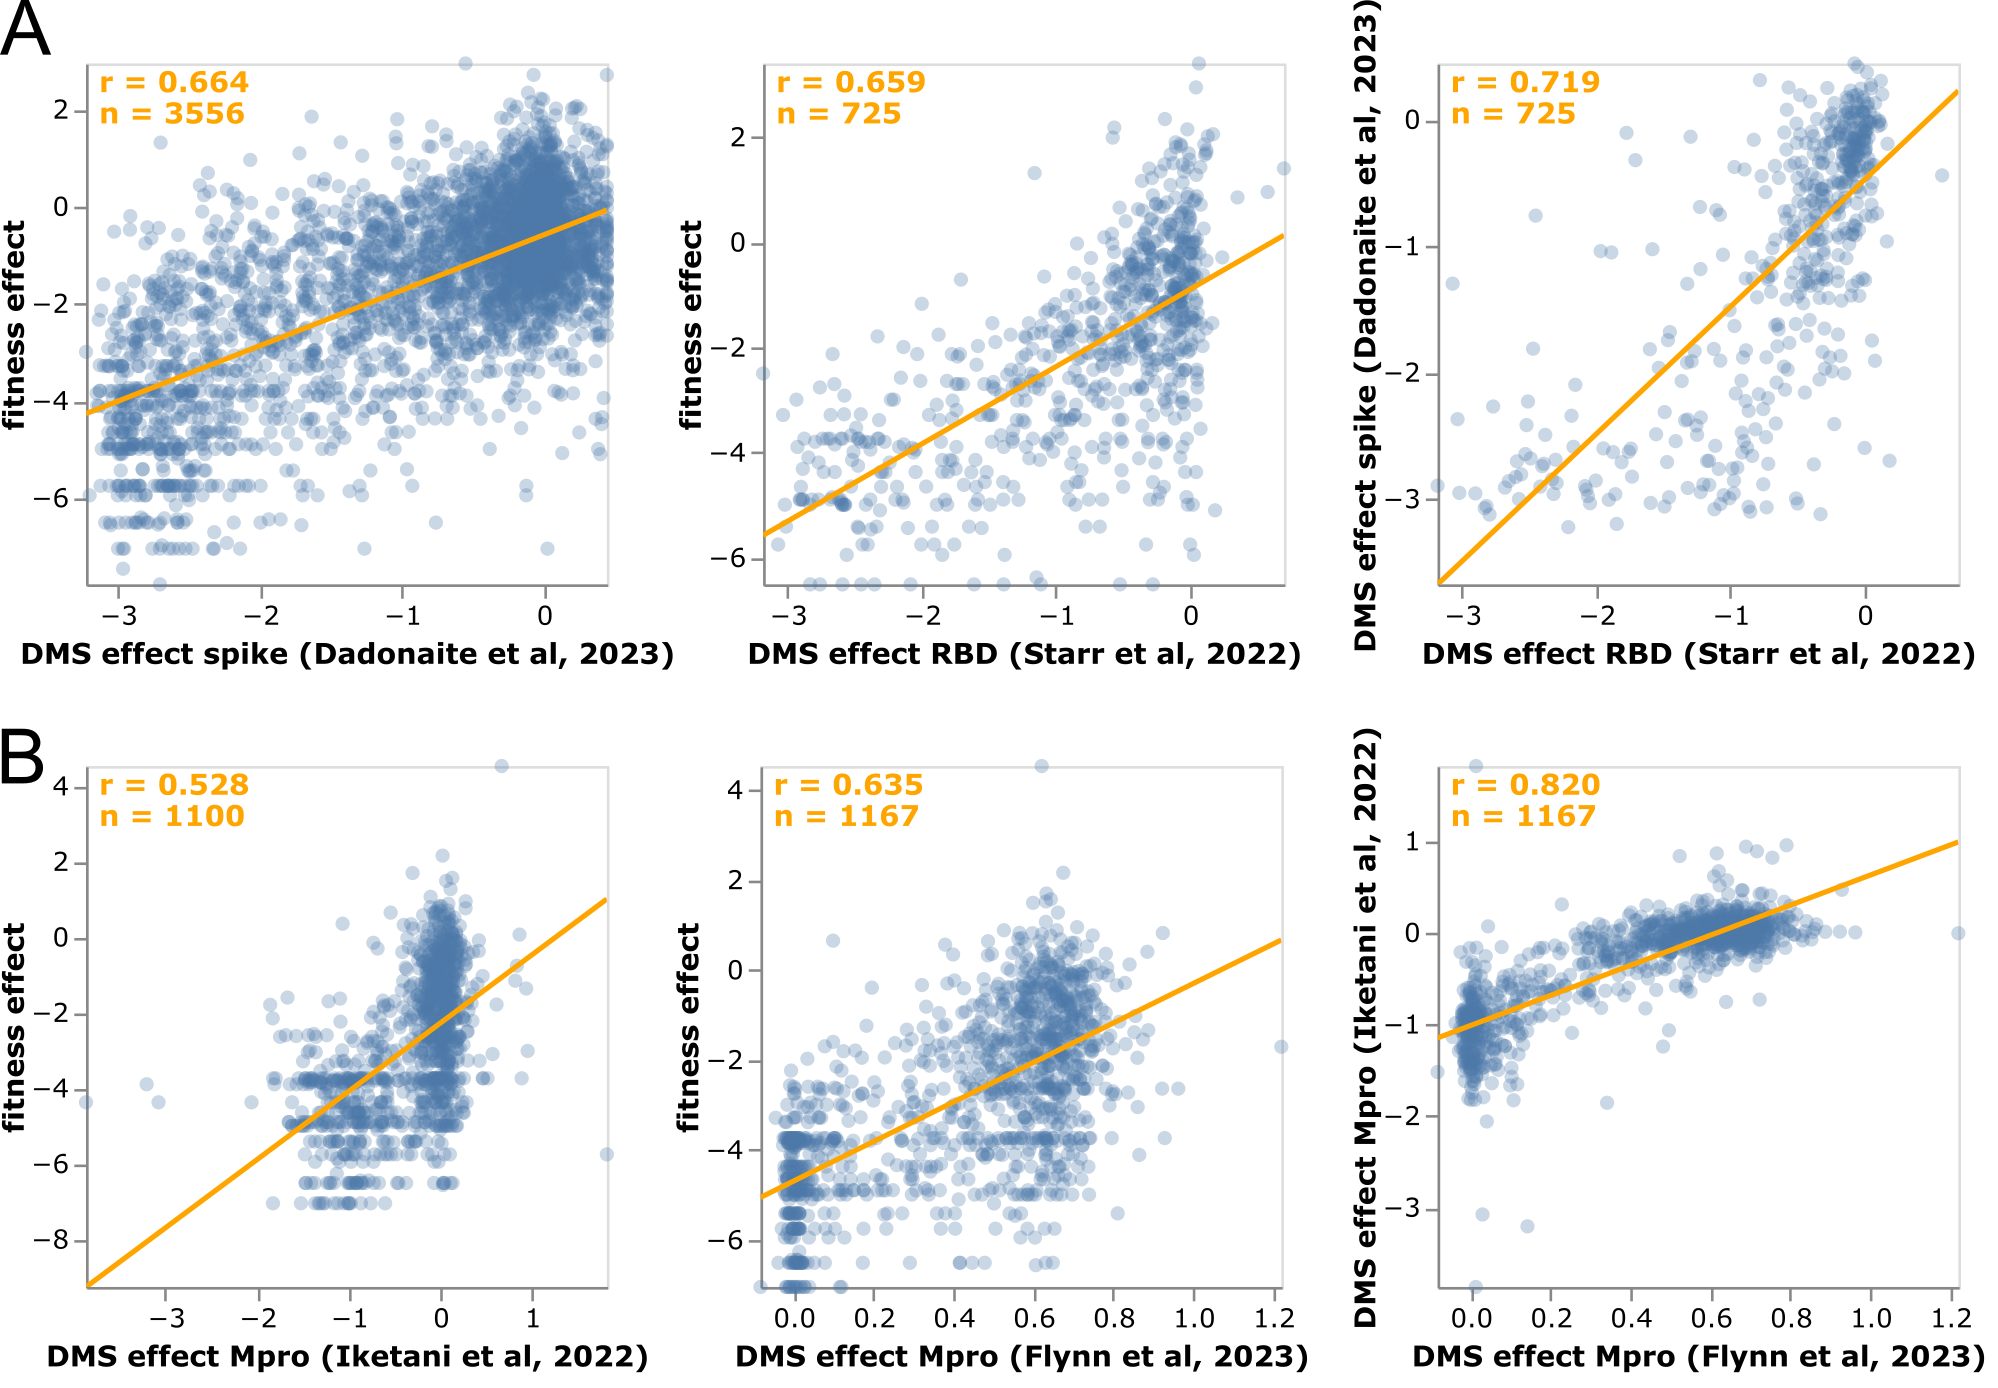
\includegraphics[width=0.7\linewidth]{figs/dms.png}
\caption{
Correlation of mutation-effect estimates with experimental deep mutational scanning measurements for {\bf (A)} the full spike~\citep{dadonaite2022pseudovirus} or its RBD~\citep{starr2022deep}, and {\bf (B)} Mpro~\citep{flynn2022,iketani2022functional}.
Each point is an amino-acid mutation, and orange text in the upper left shows the number of mutations and Pearson correlation coefficient.
Each sub-panel shows a different set of mutations (depending on which mutations were measured in that experiment).
See \url{https://jbloomlab.github.io/SARS2-mut-fitness/dms_S_corr.html} and \url{https://jbloomlab.github.io/SARS2-mut-fitness/dms_nsp5_corr.html} for plots that enable subsetting on just mutations shared across all datasets and other interactive options such as mousing over points to see mutation identities.
\label{fig:dms}
}
\end{figure*}

We examined how the mutation effects estimated using our approach compare with prior high-throughput deep mutational scanning measurements.
For spike, two distinct experimental methodologies have been used to characterize large numbers of mutations: yeast display of the receptor-binding domain (RBD)~\citep{starr2020deep,starr2022deep} and spike pseudotyped lentiviruses~\citep{dadonaite2022pseudovirus}.
For Mpro (also known as nsp5 or 3CLpro), two different labs have performed deep mutational scanning using the same basic methodology of assaying protease cleavage in yeast~\citep{flynn2022,iketani2022functional}.

For spike, our estimates from natural sequences correlate with each set of experiments almost as well as the two experimental methodologies correlate with each other (Figure~\ref{fig:dms}A).
If we increase the minimum expected counts from 10 to 20 and subset only on mutations shared among all three data sets, then the correlations between the estimates and experiments ($r = 0.66$) become even closer to the cross-experiment correlations ($r = 0.72$; see interactive version of Figure~\ref{fig:dms}A linked in legend).
Some of the mutations with the greatest divergence between our sequence-based estimates and the deep mutational scanning likely represent experimental artifacts.
For instance, P527L, which is favorable in the RBD deep mutational scan but deleterious in the sequence-based estimates and full-spike scan, is at the C-terminus of the yeast-displayed RBD~\citep{starr2020deep} where it may adopt a non-native conformation.

The sequence-based estimates for Mpro also correlate with the deep mutational scans for that protein, although in this case the two experiments correlate substantially better with each other than with our estimates (Figure~\ref{fig:dms}B).
Because both Mpro experiments use a similar yeast-based methodology~\citep{flynn2022,iketani2022functional} it is possible that the higher correlation of the experiments with each other than the sequence-based estimates reflects shared artifacts of the yeast experiments.
In particular, some Mpro mutations estimated to have deleterious effects in natural sequences are well tolerated in the yeast experiments.
This difference could arise if the yeast experiments only capture some of the constraints on Mpro in the context of actual virus.
For instance, a stop codon at Q306 is well tolerated in both deep mutational scans but extremely disfavorable in our sequence-based estimates, and would be highly deleterious to actual virus as it would truncate the polyprotein.
Similarly, K61N is well tolerated in the deep mutational scans but extremely disfavorable in our estimates, possibly because in the full viral polyprotein this residue mediates important interactions between Mpro and nsp7-10~\citep{yadav2022biochemical}

\subsection*{Interactive exploration of amino-acid fitnesses}

\begin{figure*}
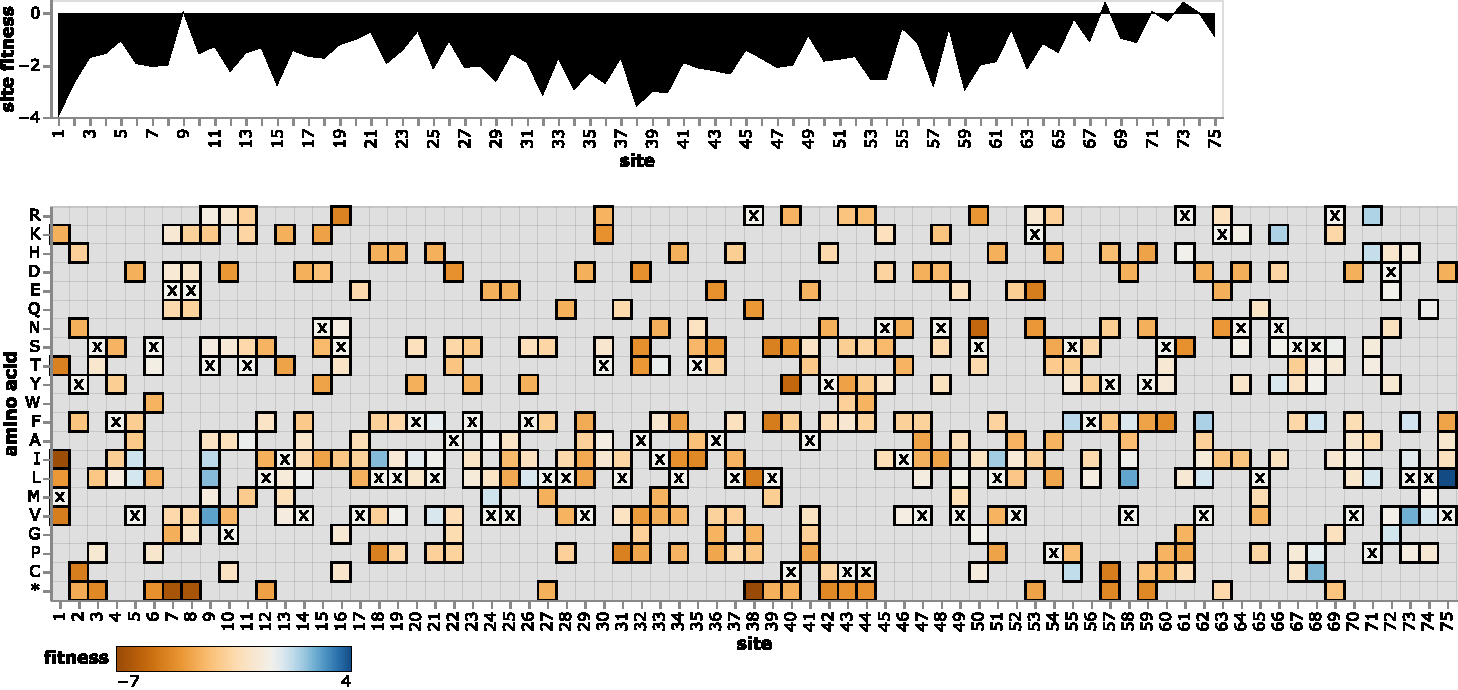
\includegraphics[width=\linewidth]{figs/E_heatmap.pdf}
\caption{
Effects of amino-acid mutations to E protein.
The area plot at top shows the average effects of mutations at each site, and the heatmap shows the effects of specific amino acids, with \textbf{x} denoting the amino-acid identity in the Wuhan-Hu-1 strain.
See \url{https://jbloomlab.github.io/SARS2-mut-fitness/E.html} for an interactive version of this plot that enables zooming, mouseovers, adjustment of the minimum expected count threshold, and layering of stop codon effects on the site plot.
See \url{https://jbloomlab.github.io/SARS2-mut-fitness} for comparable interactive plots for all SARS-CoV-2 proteins.
\label{fig:E_heatmap}
}
\end{figure*}

To enable easy access to the mutation-effect estimates, we created an interactive plots to enable exploration of the data for each protein.
A static view of one of these plots is in Figure~\ref{fig:E_heatmap}; see \url{https://jbloomlab.github.io/SARS2-mut-fitness} for interactive versions for all proteins.
These plots enable both high-level inspection of functional constraint across each protein, and detailed interrogation of the effects of specific mutations.

\section{Discussion}

We have described a new approach that estimates effects of mutations to SARS-CoV-2 by leveraging the fact that every single-nucleotide change has independently occurred many times along the evolutionary history of sequenced viruses.
In essence, we treat natural evolution as a deep mutational scan, with the millions of publicly available SARS-CoV-2 sequences from around the world providing a readout of this experiment.
The key is simply to calculate how many times each mutation has been ``tested'' along the history of sampled viral sequences, and compare that expectation to the actual counts of the mutation among viruses sufficiently fit to have been sequenced in actual human infections.

The resulting estimates of mutational effects are robust to subsetting on specific viral clades or geographies, and correlate well with prior experiments.
In broad strokes, the mutation effects illuminate patterns of constraint: for instance, while there is strong selection on structural and non-structural proteins, there is only limited purifying selection on the accessory proteins.

However, the real value of our approach is in the detailed maps of effects of specific mutations to all viral proteins, including proteins with important but poorly understood functions that are not easily characterized in the lab.
These maps will be of value for designing drugs that target constrained sites, interpreting the consequences of mutations observed during viral surveillance, and guiding experiments to better understand the functions of viral proteins.

There are several caveats to our approach.
First, because the number of occurrences of any given mutation is small compared to the millions of SARS-CoV-2 sequences being analyzed, our approach is sensitive to sequencing (or base-calling) errors as low as ~0.001\% per site.
Here we have attempted to remove spurious mutations, but further quality control is an important area for future work.
Second, we assume the rate of each type of nucleotide mutation is uniform across the viral genome, and neglect higher-order context that may influence mutation rate~\citep{sadykov2021short,beale2004comparison}.
Likewise, we neglect constraint on nucleotide identity beyond the encoded protein sequence~\citep{huston2021comprehensive,kuo2013functional}. 
Third, the exact relationship between the statistics we calculate and viral fitness depend on both the fraction of all infections that are sequenced (sampling intensity) and viral population dynamics.
Although we derive this relationship in the Methods, we do not adjust for sampling intensity and population dynamics across time and space when estimating mutation effects.
Fourth, we make a single estimate for each mutation across all SARS-CoV-2, thereby neglecting the epistasis that has affected some mutations in at least the spike protein~\citep{starr2022shifting,moulana2022compensatory}.
Finally there are a few technical caveats to how we count mutations that are discussed in the Methods section.

Conceptually, our approach differs from prior methods that aim to identify beneficial mutations associated with viral clades that expand in relative frequency~\citep{obermeyer2022analysis,lee2022inferring,maher2022predicting}.
Those methods draw information primarily from what happens downstream from a mutation.
In contrast, our approach treats all mutations equivalently regardless of whether they are on a tip node or at the base of a large clade.
Our approach is probably better for estimating the effects of deleterious or nearly neutral mutations, but clade-growth methods may be better for beneficial mutations.
In particular, clade size carries information beyond that contained in mutation counts alone (see Figure~\ref{fig:terminal}).
Hopefully future work can combine the strengths of our approach and clade-growth methods for even better estimates of mutation effects.

The power of the approach we have described will increase with growth in viral sequencing.
SARS-CoV-2 is the first virus with enough sequences that every tolerated mutation is observed multiple independent times.
As costs drop, it is easy to imagine a future with even more viral sequences.
As this occurs, viral genomic sequencing---which has traditionally been primarily a tool to track evolution and spread---will also become a means to answer questions about the effects of mutations that have traditionally required laboratory experiments.
 

{\small

\section{Methods}
\subsection{Code and data availability}
See the GitHub repository at \url{https://github.com/jbloomlab/SARS2-mut-fitness} for the computer code and processed data (eg, fitness estimates and mutation counts).
That repository contains a README with links to specific data files as well as a description of the computational pipeline.
See \url{https://github.com/jbloomlab/SARS2-mut-fitness/blob/main/results/aa_fitness/aa_fitness.csv} final estimates of amino-acid fitnesses across all clades; other intermediate data files are also provided in the GitHub repository.
The specific version of the repository used for this paper is tagged at \jdbcomment{add link to GitHub tag on final commit}.
The pipeline is fully reproducible, and is run using \texttt{snakemake}~\citep{molder2021sustainable} with interactive plots rendered using \texttt{altair}~\citep{vanderplas2018altair}.

The interactive plots are rendered at \url{https://jbloomlab.github.io/SARS2-mut-fitness} via GitHub pages.

\subsection{Counting mutations along the phylogenetic tree}
We counted occurrences of each mutation in each viral clade using the UShER pre-built mutation-annotated tree~\citep{mcbroome2021daily,turakhia2021ultrafast,lanfear2020} from Dec-18-2022 (\url{http://hgdownload.soe.ucsc.edu/goldenPath/wuhCor1/UShER_SARS-CoV-2/2022/12/18/public-2022-12-18.all.masked.nextclade.pangolin.pb.gz}), which contains all $\sim$6.5-million SARS-CoV-2 sequences that are available in public databases.
To make these counts at a per-clade level, we first subsetted the mutation-annotated tree on all sequences for each Nexstrain clade~\citep{aksamentov2021nextclade}, retained only clades with at least $10^4$ sequences, and then used the matUtils program distributed with UShER to extract the nucleotide mutations on every branch of the each clade-subsetted mutation-annotated tree.
For the analyses by geographic location (Figure~\ref{fig:corr}), we subsetted on all sequences that began with ``USA'' or ``England'' as these were the two locations with the most publicly available sequences.

We then performed quality control by ignoring any branch that met any of the following criteria:
\begin{itemize}
\item it had more than four nucleotide mutations;
\item it contained more than one nucleotide mutation that was a reversion to the Wuhan-Hu-1 reference sequence;
\item it contained more than one nucleotide mutation that was a reversion to the founder sequence for that clade as provided at \url{https://raw.githubusercontent.com/neherlab/SC2_variant_rates/7e738194a8c6592082f1caa9a6ca70cb68289790/data/clade_gts.json} by \cite{neher2022contributions};
\item it contained more than one nucleotide mutation to the same codon.
\end{itemize}
The rationale for the first exclusion is that highly mutated branches are often indicative of sequencing errors, and the rationale for the second and third exclusions is that excess reversions can arise from base-calling pipelines that erroneously call low-coverage sites as reference.
We ignore branches with multiple nucleotide mutations to the same codon (this is very rare) because as detailed below our method is only designed to make estimates for mutations that represent single-nucleotide changes from the clade founder.
Note also that the mutation-annotated tree does not include insertion or deletion mutations, and so we only consider (and make estimates for) point mutations.

We then specified for exclusion certain mutations and sites that are prone to sequencing or base-calling errors.
Specifically, we excluded
\begin{itemize}
\item the sites specified in Table S1 of \cite{turakhia2020stability} as being error prone;
\item sites 5629, 6851, 7328, 28095, and 29362 since they had very high error rates in some clades;
\item the problematic sites listed at \url{https://github.com/W-L/ProblematicSites_SARS-CoV2}, which are masked in the pre-built mutation-annotated tree;
\item for each clade, the clade-specific sites listed in \url{https://github.com/jbloomlab/SARS2-mut-fitness/blob/main/data/usher_masked_sites.yaml}, which are masked in the pre-built mutation-annotated tree;
\item for each clade, any mutation that was a reversion from the clade founder to the Wuhan-Hu-1 reference, and the reverse complements of these mutations.
\end{itemize}
The last exclusion criteria is because some bioinformatics pipelines called low-coverage sites as reference.

See \url{https://github.com/jbloomlab/SARS2-mut-fitness/blob/main/results/mutation_counts/aggregated.csv} for the final counts of each nucleotide mutation in each clade; note that this file also contains excluded mutations.

\subsection{Calculation of expected counts}
To calculate the expected counts for each nucleotide mutation, we analyzed just the four-fold degenerate sites in each clade in an approach paralleling that of \cite{bloom2022evolution}.
Specifically, we identify all non-excluded four-fold degenerate sites in each clade founder.
We then count nucleotide mutations just at those sites in each clade, and calculate the expected per-site number of mutations from nucleotide $x$ to $y$ as the total number of $x$ to $y$ mutations at four-fold degenerate sites divided by the number of four-fold degenerate sites with $x$ as the parental identity.
This analysis is done at the clade level for two reasons: referencing mutations to the clade founder (rather than the Wuhan-Hu-1 reference) limits problem with the approach that would arise at sites that substitute multiple times in the history of a sequence (since each clade is a relatively high-identity group multiple mutations at the same site within a clade are very rare), and because it is know that SARS-CoV-2 mutation rates vary somewhat among clades~\citep{bloom2022evolution,ruis2022mutational}.
We only retain clades with at least 5000 mutations at four-fold degenerate sites in order to avoid inaccurate estimates of expected counts due to low sampling of mutations.

\subsection{Mutational effects from actual versus expected counts}
To estimate the effects of mutations, we simply compare the expected counts of each nucleotide mutation to the actual counts in the pre-built mutation-annotated tree.
See \url{https://github.com/jbloomlab/SARS2-mut-fitness/blob/main/results/expected_vs_actual_mut_counts/expected_vs_actual_mut_counts.csv} for these expected versus actual counts on a per-clade basis; note that this file also includes counts at excluded sites.

To estimate the effects of mutations, we first sum the counts of all non-excluded nucleotide mutations that encode each amino-acid mutation to convert the nucleotide counts to amino-acid counts.
In doing this, we exclude any mutations that are not from the clade-founder codon identity: in other words, we ignore sequences with histories that involve multiple mutations at the same codon in the same clade (this is a caveat of the approach, although because each clade is relatively high identity it does not have a major effect).
For the overall estimates reported in this paper, we also sum these counts across all retained clades; for the analyses in Figure~\ref{fig:corr} we also make estimates without summing across clades and only for counts from sequences from specific geographic locations.
We then compute the estimated fitness $\Delta f$ of each mutation as simply the natural logarithm of the ratio of actual to expected counts after adding a pseudocount of $P - 0.5$ to each count, namely $ \Delta f = \log \left(\frac{n_{actual} + P}{n_{expected} + P}\right)$.

Note that these mutation-effect estimates will have more statistical noise the smaller the value of the expected counts for each mutation.
Therefore, we also track the expected counts alongside the estimates.
In this paper, we only show estimates for mutations with expected counts of at least 10 unless otherwise noted.
However, the figures link to interactive legends that allow adjustment of this threshold: larger values (eg, 20 or more) will lead to slightly more accurate estimates but drop some mutations, lower values can be used if you need a noisier estimate for a mutation that has less then 10 expected counts.

See \url{https://github.com/jbloomlab/SARS2-mut-fitness/blob/main/results/aa_fitness/aamut_fitness_all.csv} for the estimates of amino-acid mutation effects across all clades, and see \url{https://github.com/jbloomlab/SARS2-mut-fitness/blob/main/results/aa_fitness/aamut_fitness_by_clade.csv} for the clade-specific estimates.
The all-clade estimates of mutation effects are what are shown in Figure~\ref{fig:dist}.

For the clade correlations plotting in Figure~\ref{fig:corr}, we only include clades with at least $5 \times 10^5$ expected counts across all sites, as only these clades have enough counts for reasonable per-clade estimates.

\subsection{Mutation effects to amino-acid fitnesses}
For the final estimates of amino-acid fitnesses shown in the heatmaps such as in Figure~\ref{fig:E_heatmap}, we need a single estimate for each amino acid.
This is straightforward for sites that have the same amino-acid identity in all clade founders: the ``wildtype'' residue shared across all clades has a fitness of zero, and all other amino acids have fitnesses equal to the effect of mutating from the ``wildtype'' to that amino acid.
However, for sites that change amino-acid identity between clade founders, things are more complicated and we need to take the extra step below.

For each clade have estimated the change in fitness $\Delta f_{xy}$ caused by mutating a site from amino-acid $x$ to $y$, where $x$ is the amino acid in the clade founder sequence.
For each such mutation, we also have $n_{xy}$ which is the number of expected mutations from the clade founder amino acid $x$ to $y$.
These $n_{xy}$ values are important because they give some estimate of our "confidence" in the $\Delta f_{xy}$ values: if a mutation has high expected counts (large $n_{xy}$) then we can estimate the change in fitness caused by the mutation more accurately, and if $n_{xy}$ is small then the estimate will be much noisier.

However, we would like to aggregate the data across multiple clades to estimate amino-acid fitness values at a site under the assumption that these are constant across clades.
Things get complicated if not all clade founders have the same amino acid identity at a site.
For instance, let's say at our site of interest, the clade founder amino acid is $x$ in one clade and $z$ in another clade.
For each clade we then have a set of $\Delta f_{xy}$ and $n_{xy}$ values for the first clade (where $y$ ranges over the 20 amino acids, including stop codon, that aren't $x$), and another set of up to 20 $\Delta f_{zy}$ and $n_{zy}$ values for the second clade (where $y$ ranges over the 20 amino acids that aren't $z$).

From these sets of mutation fitness changes, we'd like to estimate the fitness $f_x$ of each amino acid $x$, where the $f_x$ values satisfy $\Delta f_{xy} = f_y - f_x$ (in other words, a higher $f_x$ means higher fitness of that amino acid).
When there are multiple clades with different founder amino acids at the site, there is no guarantee that we can find $f_x$ values that precisely satisfy the above equation since there are more $\Delta f_{xy}$ values than $f_x$ values and the $\Delta f_{xy}$ values may have noise (and is some cases even real shifts among clades due to epistasis).
Nonetheless, we can try to find the $f_x$ values that come closest to satisfying the above equation.

First, we choose one amino acid to have a fitness value of zero, since the scale of the $f_x$ values is arbitrary and there are really only 20 unique parameters among the 21 $f_x$ values (there are 21 amino acids since we consider stops, but we only measure differences among them, not absolute values).
Typically if there was just one clade, we would set the wildtype value of $f_x = 0$ and then for mutations to all other amino acids $y$ we would simply have $f_y = \Delta f_{xy}$.
However, when there are multple clades with different founder amino acids, there is no longer a well defined "wildtype".
So we choose the most common non-stop parental amino-acid for the observed mutations and set that to zero.
In other words, we find $x$ that maximizes $\sum_y n_{xy}$ and set that $f_x$ value to zero.

Next, we choose the $f_x$ values that most closely match the measured mutation effects, weighting more strongly mutation effects with higher expected counts (since these should be more accurate).
Specifically, we define a loss function as
$$
L = \sum_x \sum_{y \ne x} n_{xy} \left(\Delta f_{xy} - \left[f_y - f_x\right]\right)^2
$$
where we ignore effects of synonymous mutations (the $x \ne y$ term in second summand) because we are only examining protein-level effects.
We then use numerical optimization to find the $f_x$ values that minimize that loss $L$.

Finally, we would still like to report an equivalent of the $n_{xy}$ values for the $\Delta f_{xy}$ values that give us some sense of how accurately we have estimated the fitness $f_x$ of each amino acid.
To do that, we tabulate $N_x = \sum_y \left(n_{xy} + n_{yx} \right)$ as the total number of mutations either from or to amino-acid $x$ as the "count" for the amino acid.
Amino acids with larger values of $N_x$ should have more accurate estimates of $f_x$.

See \url{https://github.com/jbloomlab/SARS2-mut-fitness/blob/main/results/aa_fitness/aa_fitness.csv} for these overall amino-acid fitness estimates.

\subsection{Site numbering and protein naming}
All sites are numbered according to the sequential Wuhan-Hu-1 reference numbering scheme, using the reference sequence at \url{http://hgdownload.soe.ucsc.edu/goldenPath/wuhCor1/bigZips/wuhCor1.fa.gz}.
The protein annotations are taken from the associated GTF at \url{http://hgdownload.soe.ucsc.edu/goldenPath/wuhCor1/bigZips/genes/ncbiGenes.gtf.gz}.
Those protein annotations refer to the polyproteins encoding the non-structural proteins as ORF1a and ORF1ab.
To convert to from ORF1ab numbering/naming to the nsp-based naming (eg, nsp1, nsp2, etc) we use the conversions specified under ``orf1ab\_to\_nsps'' in \url{https://github.com/jbloomlab/SARS2-mut-fitness/blob/main/config.yaml}, which are in turn taken from Theo Sanderson's annotations at \url{https://github.com/theosanderson/Codon2Nucleotide/blob/main/src/App.js}.

\subsection{Derivation of relationship between actual to expected count ratio and viral fitness}
The ratio of actual to expected counts that we calculate in this paper is related to the probability that we observe a viral lineage containing an occurrence of a specific mutation among sequenced human SARS-CoV-2.
This probability depends on three factors: the fitness effect of the mutation, the fraction of all SARS-CoV-2 viruses that are sequenced (sampling intensity), and the growth dynamics of the viral population.
In the supplementary appendix, we derive the approximate relationship between this probability as a function of the fitness cost $s$ and sampling intensity $\epsilon$ for deleterious mutations for both a constant and exponentially growing viral population.

We show that for a constant viral population size, the probability of observing a lineage containing a deleterious mutation with cost $s$ is roughly $\frac{\epsilon}{s + \epsilon}$ when $s^2 > \epsilon$, and more weakly dependent on $s$ for smaller fitness costs (when $s^2 < \epsilon$).
The intuitive explanation is that the average size of a mutant lineage with fitness cost $s$ is $1/s$ and we basically ask whether we sample the lineage before it disappears.
If we sample more intensely (larger $\epsilon$), whether a lineage gets sampled depends primarily on the stochastic dynamics and little on the fitness effect.
With a typical sampling intensity for SARS-CoV-2 between 1/1000 and 1/100, this means our approach is sensitive to fitness effects larger than a few percent; mutations with fitness costs smaller than that will not show an appreciable difference from neutral mutations in their ratio of actual to expected accounts.

In an exponentially growing population, the probability of observing a mutant lineage with fitness cost $s$ again scales as $\sim \frac{\epsilon}{\epsilon + s}$ if $sT>1$, where $T$ is the time over which the variant has expanded.
If $T$ is $\sim$ months, that is 20 generations, which again corresponds to $s$ of at least a few percent for $sT > 1$. 
For mutations with smaller fitness costs, the dependence scales more as $\sim \epsilon\left(1-sT\right)$.

Overall, these calculations indicate that for multiple different growth dynamics of the viral population, the ratio of expected to actual counts will scale inversely with the fitness cost of deleterious mutations for mutations with costs that exceed a few percent.
Note that the approach we use in this paper does not account for variation in sampling intensity across space or time, does not attempt to adjust for changes in viral growth dynamics over time, uses the heuristic formula of calculating the effect as the log ratio of counts, and applies this same formula to all mutations regardless of whether they are deleterious, neutral, or beneficial.
A more complete derivation might try to calculate the fitness effects from the full distribution of lineage sizes more rigorously and incorporate information about the sampling intensity and viral growth dynamics.
However, such a derivation (if possible at all) is beyond the scope of this study, and we also note that good empirical data is generally lacking to precisely account for sampling intensity and viral growth dynamics over the full span of time and space from which the sequences we analyze are drawn.
The key point of the derivations for our current study is simply that our approach should be sensitive to detecting the effects of mutations with fitness costs greater than a few percent.

\section{Acknowledgments}
We thank Angie Hinrichs for assistance with resolving questions related to use of the UShER package and its pre-built mutation-annotated tree \jdbcomment{or add here as co-author}.
\jdbcomment{Jesse to acknowledge AVIDD, CEIRR, and R01 grants.}
JDB is an Investigator of the Howard Hughes Medical Institute.

\section{Competing interests}
JDB is on the scientific advisory boards of Apriori Bio, Aerium Therapeutics, Invivyd, the Vaccine Company, and Oncorus.
JDB receives royalty payments as an inventor on Fred Hutch licensed patents related to deep mutational scanning of viral proteins.

\bibliography{references}
}

\newgeometry{left=1in, right=1in, top=48pt, bottom=60pt}
\onecolumn
\renewcommand{\thepage}{S\arabic{page}}
\setcounter{page}{1}
\renewcommand{\thefigure}{S\arabic{figure}}
\setcounter{figure}{0}

\clearpage

\section{Supplementary appendix deriving relationship between fitness cost and ratio of expected to actual counts}

With millions of SARS-CoV-2 sequences shared publicly, almost all mutations that are tolerated by the virus are observed dozens to hundreds of times.
Where on the tree and how often on the tree we observe specific mutations has information about the effects of these mutations on viral spread.
The mutation rate depends on the nucleotides involved and possibly on the sequence context and other viral determinants, but for the purpose of this derivation, we will assume the neutral rate $\mu$ is known.
If the mutation is neutral, the total number of times the mutation is observed on the tree is $\mu T$, where $T$ is the total length of the tree (assuming that the mutation never reached high frequency which is true for almost all mutations, particularly when mutations are counted on a per-clade basis relative too the clade founder as done above).

If a mutation reduces fitness, the lineages descending from branches on which this mutation happened will spread more slowly than those without this mutation.
As a result, the down-stream subclades are smaller and more short lived, which in turn means that they will be less likely to be sampled and represented in the tree.
To infer a mutation's effect on fitness, we need to calculate how the probability of observation depends on the this fitness effect.

For a mutation to be represented in the tree, one of its descendants has to be sampled and sequenced.
If the total number of descendants is $w$ and the sampling fraction is $\epsilon$, the probability that the mutation is present in the tree is
\begin{equation}
    P = 1 - e^{-w\epsilon}
\end{equation}
$W$ is a random number that depends on the realization of the transmission process, which is commonly modeled by a branching process with birth rate $b$ and death rate $d$.
The death rate here corresponds to clearing an infection, the birth rate to onward transmission. The latter is affected by the fitness cost of the mutation.

To obtain insight how the probability of observing a lineage depends on parameters, we calculate the probability $p(w, T|t)$ that a lineage had an integrated size $w = \int_t^T k(t') \; dt'$, where $t$ is the birth time of the lineage, $T$ is the current time, and $k(t')$ is the size of the lineage at time $t'$.
To calculate $p(w,T|k)$, we generalize it slightly to $p(W, T|k,t)$, where $k$ is the number of individuals at the start time $t$. This quantity obeys the following ``first-step'' equation:
\begin{equation}
    -(\partial_t - k \partial_w) p(w,T|k,t) = -k(b+d) p(w,T|k,t) + k b p(w,T|k+1,t) + k d p(w,T| k-1, t)
\end{equation}
We will solve for the Laplace transform $\hat{p}(z,T|k,t) = \int_0^\infty dw\; e^{-wz} p(w,T|k,t) = \hat{p}^k(z,T|1,t)$.
Using the identity for the derivative of the Laplace transform
\begin{equation}
    \begin{split}
        \int_0^\infty e^{-wz} \partial_w p  \; dw& = [e^{-wz} p]_0^\infty - \int_0^\infty  p \partial_w e^{-wz} \; dw = 0 + z \int_0^\infty  p e^{-wz} = z \hat{p}
    \end{split}
\end{equation}
and using $k=1$, we have
\begin{equation}
    -\partial_t \hat{p}(z,T|t) = -(b+d+z) \hat{p}(z,T|t) + b \hat{p}^2(z,T|t) + d
\end{equation}
This simplifies further to if we substitute $\phi(z,T|t) = 1 - \hat{p}(z,T|t)$.
\begin{equation}
    \begin{split}
        \partial_t \phi(z,T|t) & = -(b+d+z) (1-\phi(z,T|t)) + b (1-\phi(z,T|t))^2 + d \\
         & = -z - (b-d-z) \phi(z,T|t) + b \phi(z,T|t)^2
    \end{split}
\end{equation}
where it is important to note that the derivative is with respect to the first time point and the interval $T-t$ is shrinking with increasing $t$.

\subsection*{Constant birth and death rate}
If the fitness effect of the mutation in question is detrimental and the overall population is constant (background $b_0=d_0$), all mutant lineages will eventually die out and we can consider large $T-t$ and $\partial_t \phi(z,T|t)$.
Further define $b=b_0 - s$ and $d=d_0$ where $s$ is the fitness cost of the mutation (so larger values indicate a greater fitness cost).
The steady state generating function is then
\begin{equation}
    0 = -z - (b-d-z) \phi(z) + b \phi(z)^2
\end{equation}
with solution
\begin{equation}
    \begin{split}
        \phi(z) & = -\frac{s + z}{2(b_0 - s)} \pm \frac{\sqrt{(s+z)^2 + 4z(b_0-s)}}{2(b_0-s)} \\
        &\approx -\frac{s + z}{2b_0} \pm \frac{\sqrt{(s+z)^2 + 4z b_0}}{2b_0} \\
        & \approx \begin{cases}
            \frac{z}{s+z} & (s+z)^2 \gg 4zb_0 \\
            \sqrt{\frac{z}{b_0}}\left(1+\frac{(s+z)^2}{8zb_0}\right)-\frac{s + z}{2b_0}  & (s+z)^2 \ll 4zb_0 \\
        \end{cases}
    \end{split}
\end{equation}
Since $\phi(z) = 1 - \int e^{-wz}p(w) \; dw$, $\phi(\epsilon)$ is exactly the probability that a lineage is sampled when the entire population is sampled at rate $\epsilon$.
We thus expect two regimes: if the square of the fitness cost exceeds the sampling intensity (typically at 1\% or less), the probability of sampling a lineage is essentially inversely proportional to the fitness cost.
The sampling probability of lineages with smaller costs effects depends less strongly on $s$.
Their sampling mostly comes down to stochasticity independent of the fitness cost.

\subsection*{Growing populations}
In many scenarios relevant for lineages that arise during a viral outbreak, the background population isn't constant but is undergoing a rapid exponential expansion.
The background birth rate $b_0$ is bigger than $d_0$ in this case.
Since the population is growing, deleterious mutations can increase in frequency deterministically and we can not send the $t$ to infinity as before.
Instead, we need to integrate
\begin{equation}
    \begin{split}
        \partial_t \phi(z,T|t) & = -z - (b-d-z) \phi(z,T|t) + b \phi(z,T|t)^2
    \end{split}
\end{equation}
backwards in time starting from $\phi(z,T|T)=0$ at $t=T$.
While $\phi(z,T|t)$ is small, this is approximately solved by
\begin{equation}
\begin{split}
    \phi(z,T|t) & = z e^{\int_t^T (b-d-z)dt'} \int_t^T e^{-\int_\tau^T (b-d-z)dt'} d\tau \\
    & = z e^{(b-d-z)(T-t)} \int_t^T e^{-(b-d-z)(T-\tau)} d\tau \\
    & = z e^{(b-d-z)(T-t)}\left[1   - e^{-(b-d-z)(T-t)}\right]/(b-d-z) \\
    & = \frac{z}{b-d-z}\left[e^{(b-d-z)(T-t)} - 1\right] = \frac{z}{\gamma_0 - s - z}\left[e^{\gamma_0 (T-t) - (s+z) (T-t)} - 1\right]
\end{split}
\end{equation}
where $\gamma_0$ is the growth rate of the background population.

At longer times when $z e^{\gamma_0 (T-t)}\sim 1$ and $\phi$ is no longer small, $\phi$ tends towards a constant value determined by the same quadratic equation as above.
This limit is neither interesting or relevant for the present purpose, since there are very few lineages that emerged early enough to have saturated $\phi$.
Instead, we need to average $\phi$ (the linear approximation) over all the time points when the lineage could have arisen.
\begin{equation}
    \begin{split}
        \langle \phi \rangle &\sim \int_t^T dt' \; e^{-\gamma_0(T-t')} \frac{z (e^{\gamma_0(T-t') - (s+z)(T-t')}-1)}{(\gamma_0 - s - z)}\\
        &= \int_t^T dt' \;  \frac{z (e^{-(s+z)(T-t')}-e^{-\gamma_0(T-t')})}{(\gamma_0 - s - z)}\\
        &\approx \begin{cases}
            \frac{z}{\gamma_0-s-z} [ \frac{1}{z+s} - \frac{1}{\gamma_0}] & s(T-t)\gg 1\\
            \frac{z}{\gamma_0-s-z} [ (T-t) - \frac{(s+z)(T-t)^2}{2} - \frac{1}{\gamma_0}] & s(T-t)<1 \\
        \end{cases}
    \end{split}
\end{equation}
This derivation assumed that $\gamma_0(T-t)\gg1$, i.e.~that the overall population size has expanded substantially.
The most relevant fitness effects will be those with $s(T-t)>1$ but $\gamma_0>s$ such that the mutant lineage has been amplified but its fitness difference to the background is a perturbation.
In this case, the above simplifies to
\begin{equation}
    \langle \phi \rangle \approx \frac{z}{\gamma_0(z+s)}
\end{equation}


In a variant that has been growing with rate $\gamma_0$ for a time $\tau=T-t$ and sampled with $z=\epsilon$, we thus expect that the number of times we observe separate mutant lineages depends on $s$ as
\begin{equation}
    \langle \phi \rangle \approx \frac{\epsilon}{\gamma_0(\epsilon+s)}
\end{equation}
This has a very similar behavior as the solution for constant population size, which suggests that the overall dependence on $s$ is robust and we can assume that the number of times a mutation is observed is inversely proportional to its effect on fitness.
In a constant population, this relationship breaks down for dense sampling $\epsilon > \sqrt{s}$.
In growing population, the approximation fails if the product of fitness effect and the time over which the variant has grown, $s\tau$, is large, i.e., if the fitness cost is substantial on this time scale.
Outside this parameter range, there is still a dependence on $s$, but it is weaker.

\clearpage

\section{Supplementary figures}

\begin{figure*}[h]
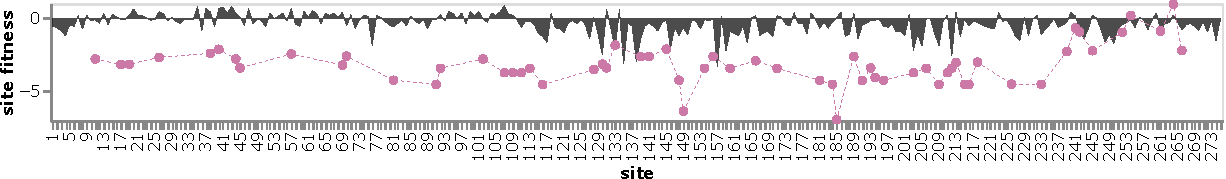
\includegraphics[width=\linewidth]{figs/ORF3a.pdf}
\caption{
Effects of stop-codon and amino-acid mutations across ORF3a.
The black area plot shows the mean effect of all amino-acid mutations at each site, and the purple points show the effects of stop codon mutations.
There is strong selection against stop codons (negative effects) for all but the C-terminus of ORF3a, but only a few positions show strong selection against amino-acid substitutions.
This plot shows only mutations with 20 expected counts.
See \url{https://jbloomlab.github.io/SARS2-mut-fitness/ORF3a.html} for an interactive version of this plot along with zoomable heatmap of the effects of specific amino-acid substitutions.
\label{fig:ORF3a}
}
\end{figure*}

\begin{figure*}
\centering
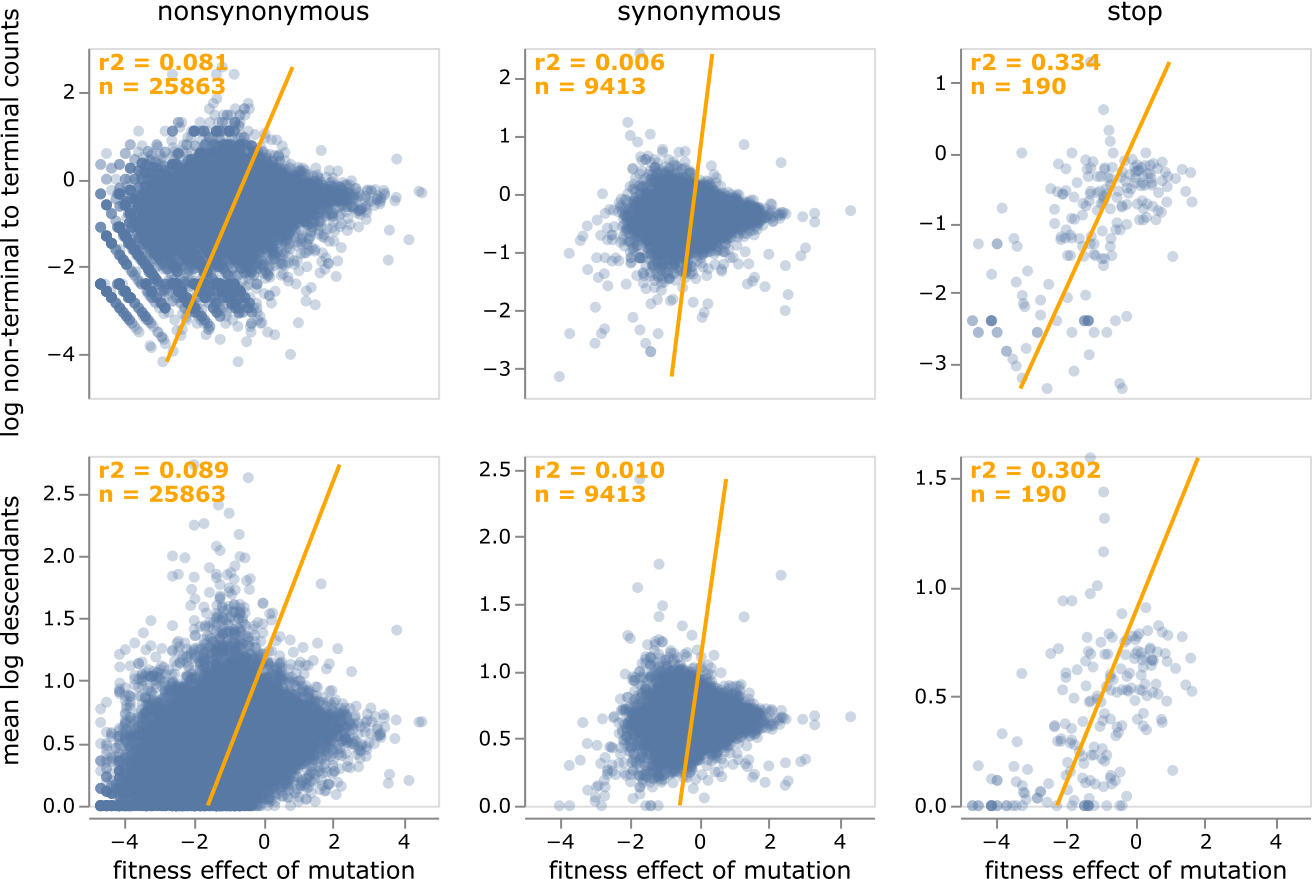
\includegraphics[width=0.75\linewidth]{figs/terminal.png}
\caption{
Relationship between fitness effects of mutations and two measures of the number of descendants.
At top is shown the log ratio of counts of the mutation on non-terminal (internal) to terminal (tip) branches; larger values indicate mutations more likely to be found in viruses that leave descendants.
At bottom is shown the mean log number of tip descendants that share all the mutations on each branch containing the mutation of interest; larger values again indicate mutations more likely to be found in viruses that leave more descendants.
Each point is an amino-acid mutation, and the orange text in the upper left give the number of mutations and the Pearson correlation coefficient.
This plot shows only mutations with at least 10 expected counts and 5 actual counts.
See \url{https://jbloomlab.github.io/SARS2-mut-fitness/fitness_vs_terminal.html} for an interactive version of this plot that allows filtering by the number of actual or expected counts, or by gene.
The number of descendants is calculated using the ``leaves\_sharing\_mutations'' variable of the UShER mutation-annotated tree.
\label{fig:terminal}
}
\end{figure*}

\begin{figure*}
\centering
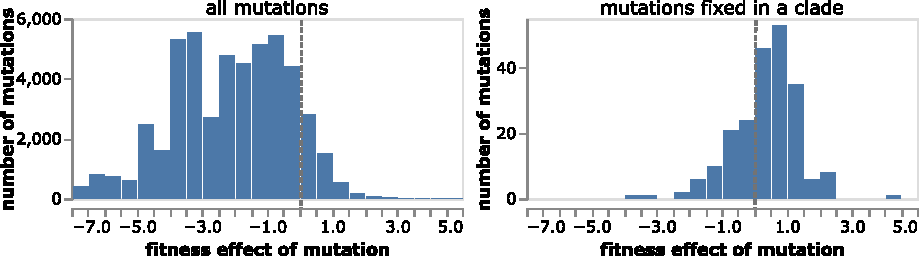
\includegraphics[width=0.7\linewidth]{figs/fixed_dist.pdf}
\caption{
\jdbcomment{Right now this figure is not reference in text; should we keep it somehow?}
Distribution of fitness effects of all amino-acid mutations relative to Wuhan-Hu-1, and all mutations that fixed in at least one clade of SARS-CoV-2 (using the Nextstrain clade definitions).
The vertical dashed line at zero indicates the effect of a neutral mutation.
Estimates are only shown for mutations with expected counts of at least 10.
See \url{https://jbloomlab.github.io/SARS2-mut-fitness/clade_fixed_muts_hist.html} for an interactive version of this plot that allows adjustment of the minimum expected count threshold.
\label{fig:fixed_dist}
}
\end{figure*}

\begin{figure*}[b]
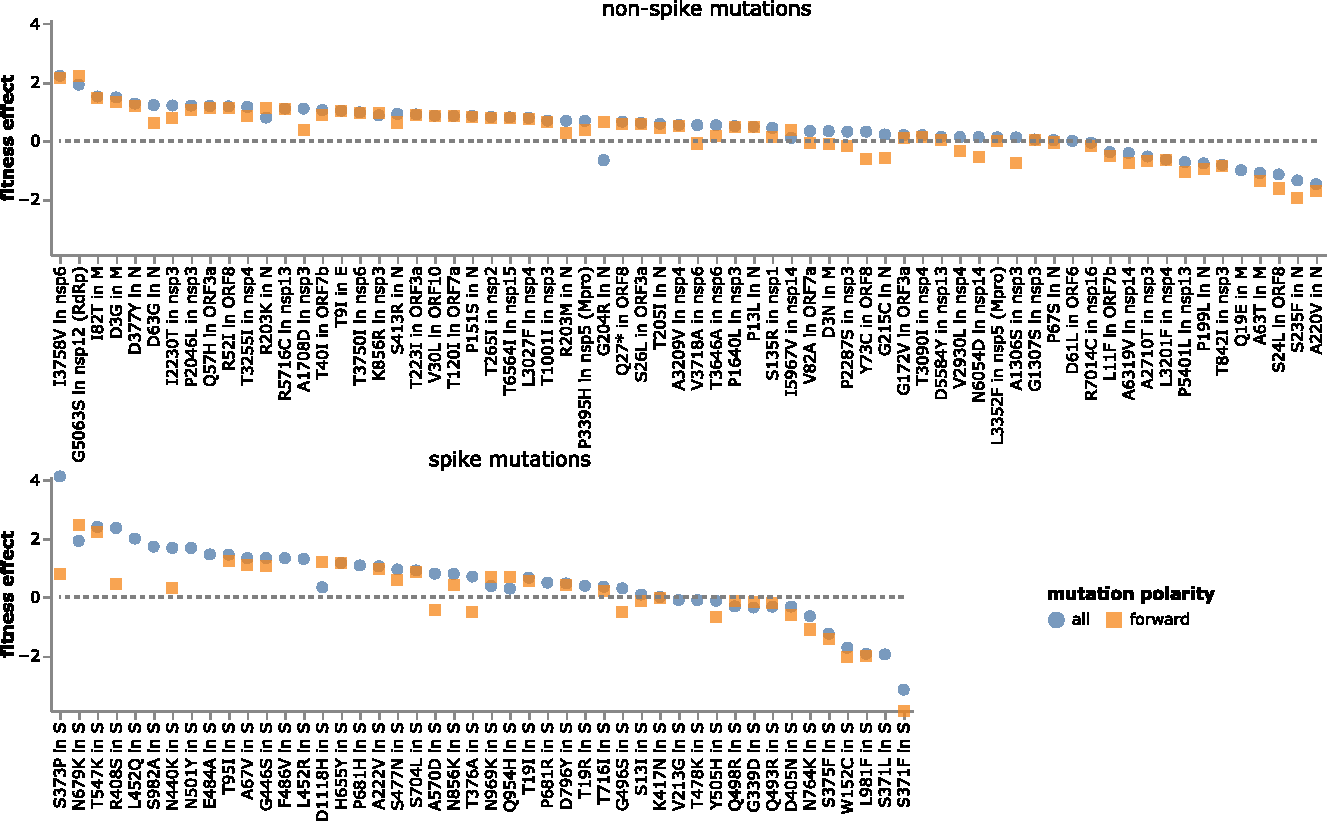
\includegraphics[width=\linewidth]{figs/fixed.pdf}
\caption{
\jdbcomment{Right now this figure is not reference in text; should we keep it somehow?}
Effects of individual mutations that fixed in at least one clade of SARS-CoV-2, faceted by whether they are in spike or another protein.
Plots show estimates of effects of mutations made across all clades (including those that have fixed the mutation) and just from direct forward occurrences of the mutation in clades in which it has not yet fixed.
Estimates are only shown for mutations with expected counts of at least 10.
See \url{https://jbloomlab.github.io/SARS2-mut-fitness/clade_fixed_muts.html} for an interactive version of this plot.
\label{fig:fixed}
}
\end{figure*}

\end{document}
